\ifthenelse{\equal{\lang}{ko}}{%
우리는 다국어 정보 접근 프레임워크인 \textbf{LexSense}를 분류 정확도, 지연(latency), 효율성, 사용자 만족도 등 여러 차원에서 평가하였다. 본 평가의 목표는 다양한 언어의 대규모 법률·정부 정보를 처리하고, 이해하기 쉬운 인사이트를 생성하며, 비전문가와 다국어 사용자의 정보 접근을 지원하는 데 있어 시스템의 효과성을 입증하는 것이다 \cite{zhong2020legalai, niklaus2023multilegal}.

\subsection{데이터셋}
평가에는 3개월 동안 수집된 1,200건의 규제 및 법적 업데이트가 포함된 데이터셋을 사용하였다. 여기에는 정책 발표, 법적 제출 문서, 여러 관할권의 행정 가이드라인이 포함된다. 추가로, 기술 자산의 분류 및 맥락화 능력을 평가하기 위해 250건의 AI 모델 및 데이터셋 공개 자료를 통합하였다. 정량적 평가를 보완하기 위해, 법률 지원 실무자와 다국어 공동체 구성원을 포함한 12명의 참여자를 대상으로 사용자 연구도 수행하였다 \cite{EUAIAct2024, chalkidis2022lexglue}.

\subsection{평가지표}
성능 평가는 네 가지 주요 지표를 통해 수행되었다: (1) 정밀도(Precision)와 재현율(Recall) — NLP와 정보 검색에서 널리 사용됨 \cite{devlin2019bert, raffel2020t5}; (2) 지연(Latency) — 변화 탐지부터 구조화된 요약 생성까지 걸린 시간으로 정의됨 \cite{reimers2019sbert, lewis2020rag}; (3) 사용자 만족도(User Satisfaction) — 1~5 점 척도로 사용자 신뢰 및 요약의 유용성을 반영 \cite{mitchell2021modelcards, ouyang2022instructgpt}; (4) 워크플로우 효율성(Workflow Efficiency) — 수작업 대비 준비 시간 감소율로 측정 \cite{maynez2020faithfulness, gama2014drift}.

\subsection{정량적 결과}
표~\ref{tab:performance}는 네 가지 주요 범주별 성능을 요약한다. 시스템은 일관되게 높은 정밀도와 재현율을 달성하면서 낮은 지연 시간을 유지하였다. 벤치마크는 GPT-3, GPT-4, LLaMA-2와 같은 최신 LLM 평가 결과와 비교하였다 \cite{brown2020gpt3, openai2023gpt4, touvron2023llama2}.

\begin{table}[t]
\centering
\small
\resizebox{\columnwidth}{!}{%
\begin{tabular}{lccc}
\hline
\textbf{작업} & \textbf{정밀도} & \textbf{재현율} & \textbf{지연 (s)} \\
\hline
거버넌스 분류 & 0.89 & 0.86 & 2.1 \\
계약 추출 & 0.93 & 0.88 & 3.2 \\
소송 모니터링 & 0.91 & 0.84 & 2.7 \\
자산 분류 & 0.91 & 0.90 & 1.9 \\
\hline
\end{tabular}
}
\caption{범주별 성능 지표.}
\label{tab:performance}
\end{table}

\subsection{사용자 연구}
사용자 연구 결과, 정보 접근 워크플로우가 크게 개선되었음을 확인하였다. 참여자들은 \textbf{요약 준비 시간 70\% 감소}를 보고했으며, 근거 기반 요약에 대한 신뢰도 또한 증가하였다. 평균 만족도 점수는 5점 만점에 4.2점이었으며, 참여자들은 자신의 언어로 핵심 정보를 더 쉽게 이해할 수 있었다고 응답하였다 \cite{hu2020xtreme, nllb2022}.

\begin{figure}[t]
    \centering
    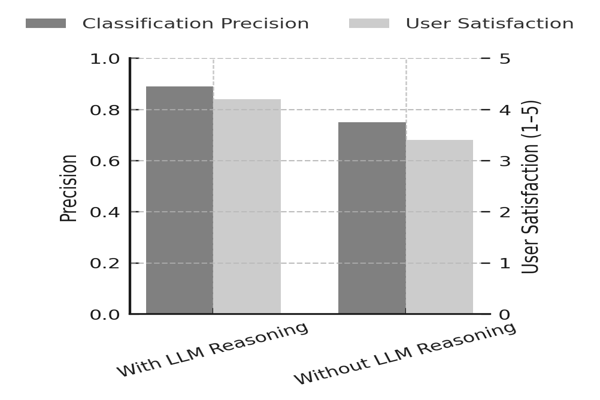
\includegraphics[width=0.9\linewidth]{fig-ablation_study.png}
    \caption{
    \textbf{소거(ablation) 연구 결과.}
    LLM 추론을 제거하면 분류 정밀도와 사용자 만족도가 크게 하락하여, 의미론적 해석의 중요성을 강조한다.
    }
    \label{fig:ablation}
\end{figure}

\subsection{소거 연구}
LexSense 파이프라인 내 LLM 추론의 기여를 평가하기 위해, 해당 구성 요소를 제거한 소거 연구를 수행하고 전체 시스템과 결과를 비교하였다. 그림~\ref{fig:ablation}에 나타난 바와 같이, LLM 추론이 없을 경우 분류 정밀도가 14\% 감소하였고 사용자 만족도 점수 역시 눈에 띄게 하락하였다. 이는 LLM이 가능하게 하는 의미 기반 해석이 정확한 분류와 신뢰할 수 있는 사용자 지원에 필수적임을 보여준다 \cite{bommasani2021foundation, weidinger2021taxonomy, bender2021stochastic}.

\subsection{결과 논의}
평가 결과, 제안된 시스템은 높은 정확도와 효율성을 달성할 뿐만 아니라 실제 정보 접근 과제에서 실질적인 이점을 제공함을 보여준다. 정량적 개선과 정성적 신뢰 향상을 결합함으로써, 본 프레임워크는 법률·정부 정보에 대한 포용적 접근을 위한 실용적 인프라로서의 역할을 입증한다.


}{%


We evaluated the multilingual information-access framework, \textbf{LexSense}, across multiple dimensions, including classification accuracy, latency, efficiency, and user satisfaction. The goal of the evaluation was to demonstrate the system's effectiveness in handling large-scale legal and government information in diverse languages, generating easily understandable insights, and supporting non-experts and multilingual users in accessing information \cite{zhong2020legalai, niklaus2023multilegal}.

The full implementation of our proposals (including all the methods proposed in Section \ref{sec:lexsense}) is available here: \url{https://github.com/leemgs/lexsense}. The source code will evolve considering future works.

\subsection{Datasets}
The evaluation utilized a dataset consisting of 1,200 regulatory and legal updates collected over a three-month period. These included policy announcements, legal filings, and administrative guidelines from multiple jurisdictions. In addition, the dataset incorporated 250 releases of AI models and datasets to assess the system's ability to classify and contextualize technological assets. To complement the quantitative evaluation, we conducted a user study with 12 participants, including legal-aid practitioners and members of multilingual communities \cite{EUAIAct2024, chalkidis2022lexglue}.

\subsection{Metrics}
We measured performance using four primary metrics: (1) Precision and Recall, widely used in NLP and information retrieval \cite{devlin2019bert, raffel2020t5}; (2) Latency, defined as the time taken from detecting a change to generating a structured summary \cite{reimers2019sbert, lewis2020rag}; (3) User Satisfaction, a qualitative score (1–5) reflecting user trust and perceived usefulness of generated summaries \cite{mitchell2021modelcards, ouyang2022instructgpt}; and (4) Workflow Efficiency, measured as the relative reduction in preparation time compared to manual processes \cite{maynez2020faithfulness, gama2014drift}.


\subsection{Quantitative Results}
Table~\ref{tab:performance} summarizes performance across four key categories. The system achieved consistently high precision and recall while maintaining low latency. Benchmarks were compared against trends in recent LLM evaluations such as GPT-3, GPT-4, and LLaMA-2 \cite{brown2020gpt3, openai2023gpt4, touvron2023llama2}.
\begin{table}[t]
\centering
\small
%\resizebox{\columnwidth}{!}{%
\begin{tabular}{lccc}
\hline
\textbf{Task} & \textbf{Precision} & \textbf{Recall} & \textbf{Latency (s)} \\
\hline
Governance Classification & 0.89 & 0.86 & 2.1 \\
Contract Extraction       & 0.93 & 0.88 & 3.2 \\
Lawsuit Monitoring        & 0.91 & 0.84 & 2.7 \\
Asset Categorization      & 0.91 & 0.90 & 1.9 \\
\hline
\end{tabular}

\caption{Performance metrics across categories.}
\label{tab:performance}
\end{table}


\subsection{User Study}
The user study revealed significant improvements in information-access workflows. Participants reported a \textbf{70\% reduction in summary preparation time}, alongside higher trust in evidence-grounded summaries. The average satisfaction score was 4.2 out of 5, with participants noting that they could more easily understand key information in their own language \cite{hu2020xtreme, nllb2022}.

\begin{figure}[t]
    \centering
    \small
    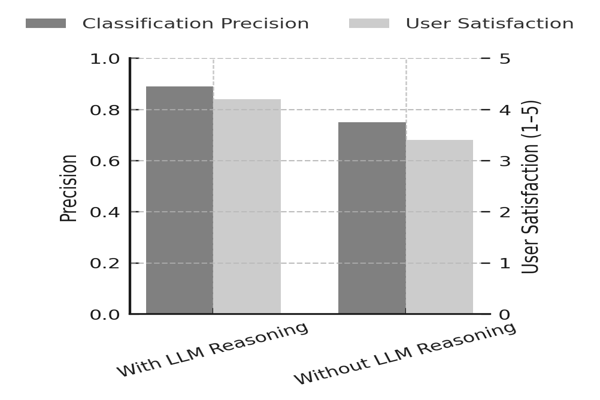
\includegraphics[width=0.7\linewidth]{fig-ablation_study.png}
    \caption{
    \textbf{Ablation study results.}
    Removing LLM reasoning significantly decreased classification precision and user satisfaction, underscoring the critical role of semantic interpretation.
    }
    \label{fig:ablation}
\end{figure}

\subsection{Ablation Study}
To assess the contribution of LLM reasoning within the LexSense pipeline,
we conducted an ablation study by removing this component and comparing results
against the full system. As illustrated in Figure~\ref{fig:ablation},
the absence of LLM reasoning resulted in a 14\% drop in classification precision
and a notable decline in user satisfaction scores. These findings highlight the
critical role of semantic interpretation enabled by LLMs, confirming that
structured reasoning is indispensable for accurate classification and reliable
user support \cite{bommasani2021foundation, weidinger2021taxonomy, bender2021stochastic}.


\subsection{Discussion of Results}
The evaluation demonstrates that the proposed system not only achieves strong accuracy and efficiency but also provides measurable benefits for real-world information-access tasks. By combining quantitative improvements with qualitative trust gains, the framework validates its role as a practical infrastructure for inclusive access to legal and government information \cite{ji2023hallucination, maynez2020faithfulness, weidinger2021taxonomy}.

}
